\documentclass{article}

% ── NeurIPS 2026 style ───────────────────────────────────────────────────────
% Options: [preprint] for arXiv, [final] for camera-ready, default = anonymous
\usepackage[preprint]{neurips_2026}

% ── Additional packages (not loaded by the sty) ──────────────────────────────
\usepackage{amsmath,amssymb}
\usepackage{booktabs}
\usepackage{xcolor}
\usepackage{graphicx}
\usepackage{microtype}
\usepackage{enumitem}
\usepackage[colorlinks=true,linkcolor=blue!60!black,citecolor=green!50!black,
            urlcolor=blue!60!black]{hyperref}
\graphicspath{{figures/}}

% ── Title ────────────────────────────────────────────────────────────────────
\title{Beyond Completion: Probing Cumulative State Tracking to Predict LLM Agent Performance}

\author{%
  Dengzhe Hou\textsuperscript{1,\dag}\hspace{1.5em}
  Lingyu Jiang\textsuperscript{1}\hspace{1.5em}
  Deng Li\textsuperscript{2}\hspace{1.5em}
  Zirui Li\textsuperscript{1}\\[2pt]
  \bf Fangzhou Lin\textsuperscript{1,3,4}\hspace{1.5em}
  Kazunori D Yamada\textsuperscript{1}\\[6pt]
  \normalfont\textsuperscript{1}Tohoku University\hspace{1em}
  \textsuperscript{2}Lappeenranta-Lahti University of Technology LUT\\[1pt]
  \textsuperscript{3}Texas A\&M University\hspace{1em}
  \textsuperscript{4}Worcester Polytechnic Institute\\[2pt]
  {\small \texttt{hou.dengzhe.t8@dc.tohoku.ac.jp}}\\[1pt]
  {\small \textsuperscript{\dag}Corresponding author.}
}

\date{}

\begin{document}

\maketitle

% ─────────────────────────────────────────────────────────────────────────────
\begin{abstract}
Task-completion rate is the standard proxy for LLM agent capability,
but models with identical completion scores can differ substantially
in their ability to track intermediate state. We introduce Working Memory Fidelity-Active Manipulation (WMF-AM), a calibrated no-scratchpad probe of cumulative arithmetic state tracking, and evaluate it on 20 open-weight models (0.5B--35B, 13 families) against a released deterministic 10-task agent battery. In a pre-specified, Bonferroni-corrected analysis, WMF-AM predicts agent performance with Kendall's $\tau{=}0.612$ ($p{<}0.001$, 95\,\% CI $[0.360,\,0.814]$); exploratory partial-$\tau$ analyses suggest this signal persists after controlling for completion score and model scale. Three construct-isolation ablations ($K{=}1$ control, non-arithmetic ceiling, yoked cancellation) support the interpretation that cumulative state tracking under load, rather than single-step arithmetic or entity tracking alone, is the primary difficulty source. K-calibration keeps the probe in a discriminative range where prior fixed-depth benchmarks become non-discriminative; generalization beyond this open-weight sample remains open.
\end{abstract}

% ─────────────────────────────────────────────────────────────────────────────
\section{Introduction}
\label{sec:intro}

This paper investigates whether a controlled probe of cumulative arithmetic state tracking captures variance in downstream agent performance not reflected by completion alone. Task-completion metrics are useful and widely applicable, but completion scores may compress variance in process-level capabilities that matter for reliable multi-step agent behavior. We call this the Completion Fallacy: the inference that completion success alone is sufficient for inferring latent process competence. Benchmarks such as HotpotQA~\citep{yang2018hotpotqa},
MMLU~\citep{hendrycks2021mmlu}, and AgentBench~\citep{liu2023agentbench}
measure what LLMs accomplish; process-sensitive probes ask \emph{how} models process information under load, a complementary evaluation lens.

We introduce and empirically validate WMF-AM, a controlled probe for
cumulative arithmetic state tracking under load, and situate it within
a working interpretive taxonomy, the Cognitive Evaluation Framework (CEF).
WMF-AM is distinguished from prior state-tracking
work~\citep{entitytracking2023,huang2025language,xia2025minerva} by
cumulative arithmetic load manipulation, targeted ablation controls,
and downstream predictive validity on a deterministic agent battery;
Section~\ref{sec:related} details the comparison.

This paper makes four contributions.
%
(1) Construct and probe.
We formalize cumulative arithmetic state tracking under load as a
measurable process-level capability and introduce WMF-AM, a
K-calibrated, no-scratchpad probe for evaluating it
(Section~\ref{sec:cef}).
%
(2) Predictive validity.
Across 20 open-weight models (0.5B--35B, 13 families), WMF-AM
predicts performance on a non-overlapping deterministic 10-task agent
battery ($\tau{=}0.612$, $p{<}0.001$, 95\,\% CI
$[0.360,\,0.814]$; pre-specified, Bonferroni-corrected;
Section~\ref{sec:pilot}).
Exploratory partial-$\tau$ analyses suggest the signal persists
after controlling for task completion and model scale.
%
(3) Construct isolation.
Three targeted ablations, a $K{=}1$ single-step control, a
non-arithmetic ceiling condition, and a yoked cancellation
control, support the interpretation that cumulative state tracking under load, rather
than single-step arithmetic or generic entity tracking, is the
primary difficulty source within this sample (Section~\ref{sec:robustness}).
%
(4) Measurement robustness.
WMF-AM rankings are stable across random seeds, prompt templates
($\tau_{\text{bare,chat}}{=}0.524$, $p{=}0.006$; pre-specified),
natural-language paraphrases, and leave-one-family-out analyses
(Section~\ref{sec:meas_robustness}).
%
\noindent A glossary of all acronyms appears in
Table~\ref{tab:glossary} (Appendix~\ref{app:glossary}).
Generalization to closed API models and broader criteria remains open;
the CEF taxonomy is an interpretive framework, not an empirical claim.
% ─────────────────────────────────────────────────────────────────────────────
\section{Related Work}
\label{sec:related}

\paragraph{Completion-based evaluation and the process-quality gap.}
Standard benchmarks, MMLU~\citep{hendrycks2021mmlu},
HotpotQA~\citep{yang2018hotpotqa}, AgentBench~\citep{liu2023agentbench},
HELM~\citep{liang2023helm}, measure outcome correctness without
probing the reasoning process.
This creates what we term the Completion Fallacy, an instance of multiple
realizability~\citep{putnam1967}: identical outcomes produced by
categorically different processes, documented also as
underspecification~\citep{damour2022underspecification} and shortcut
learning~\citep{geirhos2020shortcut}.
Within our 20-model sample, 30/105 pairs with
$|\Delta\text{completion}|\leq 0.05$ show $|\Delta\text{WMF-AM}|\geq 0.10$,
illustrating that, in this sample, completion compresses process-level variance.

\paragraph{Evidence of process-outcome dissociation.}
Recent work documents process-outcome gaps at scale.
PAE~\citep{xie2026m3} finds 27--78\% of agent successes involve
corrupted trajectories; Fragile Thoughts~\citep{aravindan2026fragile}
and Robust Answers Fragile Logic~\citep{jiang2026robustanswersfragilelogic}
show correct answers produced despite broken reasoning chains;
Turpin et al.~\citep{turpin2023language} demonstrate unfaithful
chain-of-thought explanations.
AgentProcessBench~\citep{fan2026agentprocessbench} provides 8,509
human-annotated steps showing step-level quality diverges from outcomes.
Process supervision~\citep{lightman2023verify,uesato2022solving} trains
on step-level labels; CEF measures process quality without
requiring labelled training data.

\paragraph{State-tracking and process-sensitive probes.}
A growing body of work probes how LLMs maintain and update internal
state representations.
Entity Tracking~\citep{entitytracking2023} tests passive state
retrieval (e.g., which container holds a given object after a
sequence of swaps), while Latent State
Persistence~\citep{huang2025language} extends to sequential
manipulation of hidden integers---the closest prior paradigm to
WMF-AM, though without arithmetic accumulation or downstream
agent-predictive validation.
Several recent benchmarks~\citep{rezaee2025statetracking,li2025howtrack}
similarly probe object or entity state, and Zhang et
al.~\citep{zhang2024working} motivate working-memory-style evaluation,
but none pair ablation controls with an external criterion battery.
Minerva~\citep{xia2025minerva} includes a Quantity State task that
is structurally closest to WMF-AM, sequential additive/subtractive
operations, yet its fixed depth of $K{=}200$ places all 20 of our
study models at exactly 0.000, rendering the probe non-discriminative
($\tau$ undefined).

WMF-AM addresses this gap along three axes:
K-calibration restoring discriminability across the 0.5B--35B range,
a construct-isolation ablation suite, and predictive validity against a
deterministic agent battery (head-to-head with Minerva in
Section~\ref{sec:discussion}).

% ─────────────────────────────────────────────────────────────────────────────
\section{WMF-AM and Its Interpretive Framework (CEF)}
\label{sec:cef}

CEF (Cognitive Evaluation Framework) is a design lens that organizes
process-sensitive probes into four proposed dimensions: WMF
(Working Memory Fidelity), MCC (Metacognitive Calibration),
EMC (Episodic Memory Coherence), and CLA (Cognitive Load Adaptation),
with 11 sub-dimensions.
This dimensional structure is hypothesized; factor analysis requires
$N{\geq}30$ (Appendix~\ref{app:cef_background};
glossary in Table~\ref{tab:glossary}).

\paragraph{Flagship probe: WMF-AM.}
\label{sec:wmfam_probe}
WMF-AM (Active Manipulation) is a probe of cumulative arithmetic
state tracking under load, inspired by working-memory span paradigms.
An initial numeric state is presented, $K$ sequential additive/subtractive
operations arrive, and the model must report the final cumulative state.
The pilot uses depths $K \in \{3,5,7\}$ (dissociation study) and $K
\in \{2,4,6,8,12\}$ (yoked cancellation control), across three surface
forms (points scoring, warehouse inventory, bank accounts). Prior entity
tracking~\citep{entitytracking2023} tests passive retrieval; WMF-AM
tests sequential arithmetic transformation under load.

\textbf{Scope.} WMF-AM measures difficulty with maintaining a running
cumulative sum across $K$ operations.
A $K{=}1$ control separates cumulative tracking from single-step arithmetic:
13/15 models achieve near-ceiling accuracy at $K{=}1$
($\bar{x}{=}0.957$) versus $\bar{x}{=}0.151$ at $K{=}7$,
indicating that cumulative load, not arithmetic skill per se,
is the primary difficulty driver.

\textbf{Worked example ($K{=}3$, points form):} ``Alice starts
with 10 points. Alice gains 5 points. Alice loses 3 points. Alice gains
7 points. What is Alice's current score?'' Correct answer: 19.
Scoring: exact match (1 if the model outputs 19, 0 otherwise).
A model that tracks each update cumulatively
($10 \to 15 \to 12 \to 19$) succeeds; a model that performs only the
last operation or guesses a plausible number fails. At $K{=}7$, the
chain length taxes state maintenance, producing the diagnostic
depth$\times$accuracy interaction.

\textbf{Yoked control example ($K{=}3$):} ``Alice starts with 10
points. Alice gains 5 points. Alice loses 5 points. Alice gains 3
points. Alice loses 3 points. Alice gains 7 points. Alice loses 7
points. What is Alice's current score?'' Correct answer: 10 (initial
state). Each operation is immediately followed by its inverse, requiring
identical arithmetic but no cumulative tracking.

Preliminary pilots for MCC, EMC, and CLA are reported in
Appendix~\ref{app:emclite}--\ref{app:mccv2}; construct-validity
framework and falsification criteria are in Appendix~\ref{app:falsify}.

% ─────────────────────────────────────────────────────────────────────────────
\section{Validation Study: WMF-AM Provides Initial Predictive Evidence for Agent Performance}
\label{sec:pilot}

\paragraph{Variable definitions.}
Three scores are used throughout this section and should not be confused.
\textbf{WMF-AM Score}: the probe output, mean accuracy over $K\in\{3,5,7\}$ depths,
4 random seeds, and 3 surface forms (points / inventory / accounts) for each model,
all collected under each model's Ollama default chat template (Section~\ref{sec:cef}).
Prompt-wrapper variation (bare / chat / CoT) is analyzed separately as a robustness
check in Phase~5 (Section~\ref{sec:robustness}) and is \emph{not} folded into the
primary WMF-AM Score.
(In Phase~5, ``chat'' denotes the same Ollama default chat wrapper used
for the primary evaluation; ``bare'' strips it.)
\textbf{Outcome Correctness (OC)}: the 100-item general-knowledge completion
battery used as a general-capability baseline (Section~\ref{sec:pilot},
Phase~1); this is the ``completion score'' referred to throughout.
\textbf{Agent Battery Score (ABS)}: the 10-task deterministic downstream
criterion (Phase~6); this is the ``agent score'' or ``downstream target''
used in all predictive validity analyses.
OC and WMF-AM serve as predictors; ABS is the downstream criterion.

\paragraph{Statistical methodology.}
All rank correlations use Kendall's $\tau$-b (ties accounted for).
Partial $\tau$ uses Somers residualization~\citep{somers1962new}.
Bootstrap 95\% CIs: 10{,}000 model-level and family-clustered resamples;
family-clustered CI $[0.341, 0.815]$ is virtually identical to
model-level $[0.360, 0.814]$, no single family is load-bearing
($\tau \in [0.503, 0.649]$ across leave-family-out runs). Pre-specified primary analyses (Bonferroni-corrected, $\alpha{=}0.025$):
(1)~predictive validity ($\tau = 0.612$) and (2)~template stability ($\tau = 0.524$).
Both were frozen before expansion-set collection; all other analyses are exploratory.

\paragraph{Formal criterion.}
Let $Y_i \in [0,1]$ denote the outcome score (OC) and
$Z_i \in [0,1]$ a process-sensitive measure (WMF-AM) for model~$i$.
Outcome metrics are statistically insufficient w.r.t.\
a downstream criterion $D$ if
$\text{partial}\;\tau(Z, D \mid Y) > 0$ at conventional~$\alpha$.
This condition is benchmark-specific, not a universal claim.
We report an exploratory test of this criterion in Section~\ref{sec:confirmatory}.

\begin{table}[h]
\centering
\small
\caption{\textbf{Study map: complete analysis register.}
All $\tau$ = Kendall's $\tau$-b.
\textbf{C} = pre-specified primary (Bonferroni-corrected at $\alpha{=}0.025$);
\textbf{E} = exploratory (hypothesis-generating only; require held-out replication
before drawing strong conclusions).
Predictor: WMF-AM Score; Criterion: Agent Battery Score (ABS);
Baseline: Outcome Correctness (OC).}
\label{tab:keyanalyses}
\resizebox{\linewidth}{!}{%
\begin{tabular}{@{}lp{3.2cm}ccccl@{}}
\toprule
\textbf{Relation} & \textbf{Subset} & $\tau$ & $N$ & $p$ & \textbf{95\% CI} & \textbf{Type} \\
\midrule
WMF-AM $\to$ Agent overall & All models & 0.612 & 20 & $<$0.001 & $[0.360, 0.814]$ & C \\
Bare $\leftrightarrow$ Chat template ranks & 15 models & 0.524 & 15 & 0.006 & --- & C \\
WMF-AM $\to$ Agent (partial $|$ OC) & All models & 0.411 & 20 & 0.011 & --- & E \\
WMF-AM $\to$ Agent (partial $|$ $\log$ params) & All models & 0.503 & 20 & $<$0.01 & --- & E \\
WMF-AM $\to$ Agent (partial $|$ OC $+$ $\log$ params) & All models & 0.389 & 20 & 0.016 & --- & E \\
WMF-AM $\to$ Agent non-WMF (7 tasks) & All models & 0.623 & 20 & $<$0.001 & --- & E \\
WMF-AM $\to$ Agent WMF-heavy (3 tasks) & All models & 0.527 & 20 & 0.003 & --- & E \\
WMF-AM $\leftrightarrow$ OC & 15 models & 0.279 & 15 & 0.150 & $[-0.156, 0.637]$ & E \\
CONV-RFPOC $\leftrightarrow$ AGENT-PQ & 7 models & 0.905 & 7 & 0.003 & --- & E \\
\bottomrule
\end{tabular}}
\end{table}

\paragraph{Note on sample sizes.} Different analyses use different subsets:
$N{=}20$ for all predictive validity and completion-battery analyses
(the full study set); $N{=}15$ for WMF-AM template stability and
divergent validity (original 7 + expansion 8; before small models
were added); $N{=}7$ for convergent validity only (original models
with AGENT-PQ and CONV-RFPOC data collected).
AGENT-PQ is a separate LLM-judged process-quality measure used only for
convergent validity and should not be confused with ABS (the deterministic
exact-match agent battery used as the primary downstream criterion).
All sample sizes are reported explicitly at each result.

{\sloppy
Twenty open-weight models from thirteen architectural families form the
study set: seven original models (Qwen 7B/14B/32B, Llama 3.1:8b,
Gemma 2:27b, DeepSeek-R1:14b, Mistral:7b), eight expansion models
(Phi-3:14b, Gemma-2:9b, Qwen-2.5:3b, Llama-3.2:3b, DeepSeek-R1:7b,
Mixtral:8x7b, Command-R:35b, Yi:34b), and five small baseline models
(0.5B--2B parameters; Table~\ref{tab:pilot}).
\par}
Models were evaluated in six phases. Phase~1 (Outcome Correctness)
used a 100-item battery spanning five domains (factual, math, science,
reasoning, language) at five difficulty levels, temperature $= 0$.
Phase~2 (WMF-AM) administered 15 probes at depths $K \in \{3,5,7\}$
with 4 independent random seeds for all 20 models.
Phase~3 (MCC-MA) applied a 20-problem self-monitoring probe.
Phase~4 (Yoked Cancellation Control) administered 20 trials per depth at
$K \in \{2,4,6,8,12\}$ using operations that cancel (gain then lose,
transfer then reverse), so the correct answer equals the initial state
despite requiring identical arithmetic parsing as WMF-AM.
Phase~5 (Template Harmonization) re-administered WMF-AM under three
prompt wrappers (bare, chat, chain-of-thought) to test prompt-format
sensitivity.
Phase~6 (Agent Validation) administered 10 multi-step agent tasks
(tool use, multi-step reasoning, state tracking) to all 20 models
to test predictive validity.
All models are Ollama-hosted open-weight variants using default chat
templates, fp16 quantization where available, and greedy decoding
(temperature $= 0$, no top-$p$ sampling). No task overlap exists
between phases (full study matrix in Appendix~\ref{app:studymatrix}).
Table~\ref{tab:methods} summarizes the experimental design.

\begin{table}[t]
\centering
\small
\caption{\textbf{Study design summary.} All phases: temperature $= 0$,
greedy decoding, Ollama-hosted models with default chat templates.
All 20 models evaluated with 4 seeds for WMF-AM.}
\label{tab:methods}
\resizebox{\linewidth}{!}{%
\begin{tabular}{@{}llcccl@{}}
\toprule
\textbf{Phase} & \textbf{Probe} & \textbf{Depths} & \textbf{Items} & \textbf{Seeds} & \textbf{Scoring} \\
\midrule
1.\ Outcome & 100-item battery (5 domains) & --- & 100 & 1 & Exact match (0/1) \\
2.\ WMF-AM & State tracking & $K{=}3,5,7$ & 15/depth & 4 & Exact match on final state \\
3.\ MCC-MA & Self-monitoring & --- & 20 & 1 & Pearson $r$ (predicted vs actual) \\
4.\ Yoked & Cancellation ops & $K{=}2,4,6,8,12$ & 20/depth & 1 & Exact match on initial state \\
5.\ Template & 3 prompt wrappers & $K{=}3,5,7$ & 15/depth & 1 & Rank stability ($\tau$) \\
6.\ Agent & 10 multi-step tasks & --- & 10 & 1 & Deterministic task score (0--1) \\
\bottomrule
\end{tabular}}
\end{table}

\begin{figure}[t]
\centering
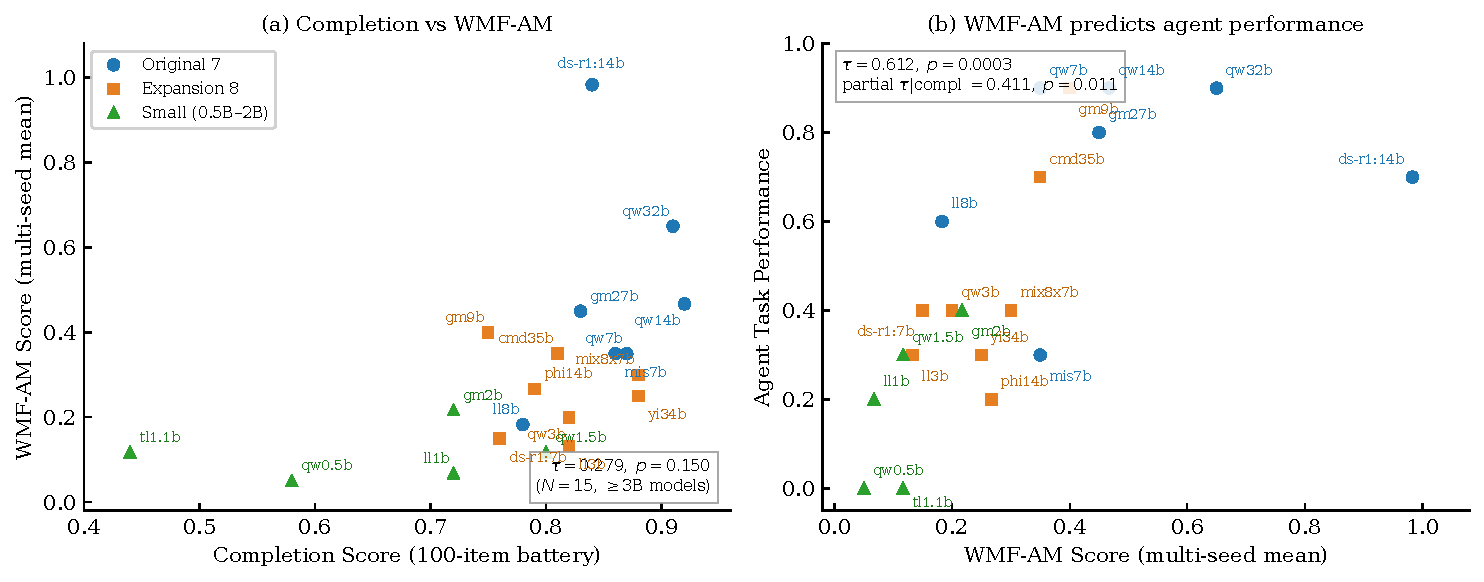
\includegraphics[width=\textwidth]{fig1_dissociation.pdf}
\caption{\textbf{(a)} Completion clusters while WMF-AM spans a wide range
($N{=}20$, 13 families). \textbf{(b)} WMF-AM predicts downstream agent
performance ($\tau{=}0.612$, $p{<}0.001$; pre-specified confirmatory).
Exploratory: partial $\tau{=}0.411$ ($p{=}0.011$) after controlling
for completion (same sample; requires held-out replication).
Blue circles = original 7; orange squares = expansion 8; green triangles = small models (0.5B--2B).}
\label{fig:dissociation}
\end{figure}

\subsection{Primary Confirmatory Results}
\label{sec:confirmatory}

\paragraph{WMF-AM predicts Agent Battery Score.}
Figure~\ref{fig:dissociation} and Table~\ref{tab:pilot} present the key
finding across $N{=}20$ models from 13 families. WMF-AM (4-seed means)
spans 0.050--0.983 ($\Delta = 0.933$) while the 100-item completion
battery spans 0.44--0.92 ($\Delta = 0.480$).
Among the 15 mid-to-large models ($\geq$3B), OC clusters
at 0.75--0.92 (SD $= 0.052$) while WMF-AM spans 0.133--0.983 (SD $= 0.228$):
OC masks substantial process-quality differences.
Predictive validity: WMF-AM significantly predicts
performance on a deterministic 10-task multi-step agent battery within this 20-model open-weight sample
($\tau = 0.612$, $p < 0.001$, $N{=}20$;
bootstrap 95\% CI $[0.360, 0.814]$).
A held-out check on llama3.1:70b (withheld from the study set)
yields $\tau = 0.627$ ($p = 0.0002$, $N{=}21$), essentially unchanged;
this is consistent with but does not constitute replication.
Exploratory incremental validity:
partial $\tau = 0.411$ ($p = 0.011$) after controlling for OC,
and partial $\rho = 0.437$ ($p = 0.008$) via Spearman (robustness check),
are consistent across two rank-correlation families (exploratory; same $N{=}20$ sample).
OC also predicts agent performance ($\tau = 0.428$, $p = 0.012$).
The primary pre-specified evidence is twofold:
(1)~significant pre-specified predictive validity ($\tau = 0.612$) and
(2)~significant pre-specified template stability ($\tau = 0.524$, $p = 0.006$).

\begin{table}[t]
\centering
\small
\resizebox{\linewidth}{!}{%
\begin{tabular}{llccccc}
\toprule
Model & Family & Outcome & WMF-AM & Agent & Yoked & WMF$-$Yoked \\
\midrule
\multicolumn{7}{l}{Original 7 (all 4-seed WMF-AM)} \\
deepseek-r1:14b & DeepSeek & 0.840 & \textbf{0.983} & 0.70 & 0.810 & $+$0.173 \\
qwen2.5:32b     & Qwen     & 0.910 & 0.650 & \textbf{0.90} & 1.000 & $-$0.350 \\
qwen2.5:14b     & Qwen     & 0.920 & 0.467 & \textbf{0.90} & 0.710 & $-$0.243 \\
gemma2:27b      & Gemma    & 0.830 & 0.450 & 0.80 & 0.620 & $-$0.170 \\
qwen2.5:7b      & Qwen     & 0.870 & 0.350 & \textbf{0.90} & 0.770 & $-$0.420 \\
mistral:7b      & Mistral  & 0.860 & 0.350 & 0.30 & 0.550 & $-$0.200 \\
llama3.1:8b     & Llama    & 0.780 & 0.183 & 0.60 & 0.340 & $-$0.157 \\
\midrule
\multicolumn{7}{l}{Expansion 8 (all 4-seed WMF-AM)} \\
gemma2:9b       & Gemma    & 0.750 & 0.400 & \textbf{0.90} & 0.960 & $-$0.560 \\
command-r:35b   & Cohere   & 0.810 & 0.350 & 0.70 & 0.920 & $-$0.570 \\
mixtral:8x7b    & Mistral  & 0.880 & 0.300 & 0.40 & 1.000 & $-$0.700 \\
phi3:14b        & Phi      & 0.790 & 0.267 & 0.20 & 0.950 & $-$0.683 \\
yi:34b          & Yi       & 0.880 & 0.250 & 0.30 & 1.000 & $-$0.750 \\
qwen2.5:3b      & Qwen     & 0.820 & 0.200 & 0.40 & 0.970 & $-$0.770 \\
deepseek-r1:7b  & DeepSeek & 0.760 & 0.150 & 0.40 & 0.940 & $-$0.790 \\
llama3.2:3b     & Llama    & 0.820 & 0.133 & 0.30 & 0.510 & $-$0.377 \\
\midrule
\multicolumn{7}{l}{Small models (broader baseline)} \\
gemma2:2b       & Gemma    & 0.720 & 0.217 & 0.40 & --- & --- \\
qwen2.5:1.5b    & Qwen     & 0.800 & 0.117 & 0.30 & --- & --- \\
tinyllama:1.1b  & TinyLlama& 0.440 & 0.117 & 0.00 & --- & --- \\
llama3.2:1b     & Llama    & 0.720 & 0.067 & 0.20 & --- & --- \\
qwen2.5:0.5b    & Qwen     & 0.580 & 0.050 & 0.00 & --- & --- \\
\midrule
$\Delta$ & — & 0.480 & \textbf{0.933} & 0.90 & — & — \\
\bottomrule
\end{tabular}}
\caption{\textbf{Per-model scores: WMF-AM Score, Outcome Correctness (OC),
Agent Battery Score (ABS), and Yoked control accuracy ($N{=}20$, 13 families).}
WMF-AM Score = 4-seed mean at $K\in\{3,5,7\}$; OC = 100-item general-knowledge
battery (Outcome Correctness; baseline predictor); ABS = 10-task deterministic
agent battery (downstream criterion; pre-specified primary analysis).
WMF-AM (pre-specified primary): $\tau{=}0.612$ ($p{<}0.001$, confirmatory, C).
OC $\to$ ABS: $\tau{=}0.428$ ($p{=}0.012$, exploratory, E).
Yoked column: cancellation-control accuracy (original 15 models only).}
\label{tab:pilot}
\end{table}

\subsection{Construct Isolation and Alternative Explanations}
\label{sec:robustness}

\paragraph{Completion battery design.}
Phase~1 uses a custom 100-item battery (five domains $\times$ five difficulty
levels; score resolution 0.01) as a within-study general-capability control,
not a standard benchmark suite. An exploratory $\log(\text{parameter count})$
control ($\tau = 0.503$, $p < 0.01$) provides a complementary proxy
independent of battery choice; the joint partial $\tau$ ($0.389$,
$p = 0.016$) controls for both simultaneously.
With the addition of 5 small models (0.5B--2B), OC ranges from
0.44 to 0.92 (SD $= 0.131$, $N{=}20$) and correlates with agent
performance ($\tau = 0.428$, $p = 0.012$); WMF-AM shows an exploratory
signal of \emph{incremental} prediction (partial $\tau = 0.411$,
$p = 0.011$).
Among the 15 mid-to-large models ($\geq$3B), OC remains compressed
(SD $= 0.052$), consistent with range restriction being a property of
the model population rather than the battery design.

{\sloppy
\paragraph{Exploratory architectural observations (Appendix~\ref{app:dissociation}).}
Only deepseek-r1:14b shows positive WMF$-$Yoked residual ($+0.173$),
suggesting genuine cumulative tracking; all other 14 models show negative
residuals, with the largest gaps in smaller models.
Figure~\ref{fig:depth} shows depth-dependent degradation curves ($N{=}15$).
\par}

\paragraph{Alternative explanations and template sensitivity.}
WMF-AM scores may reflect nuisance factors beyond state tracking:
instruction-following ability, tokenizer effects on numeric parsing,
scratchpad/chain-of-thought policy differences, or prompt-format
sensitivity. Phase~5 (template harmonization) directly tests the last
concern: across 15 models $\times$ 3 templates, model rankings under
bare and chat wrappers are significantly correlated
($\tau_{\text{bare,chat}} = 0.524$, $p = 0.006$), indicating that
WMF-AM rankings are moderately robust to prompt-format variation.
Chain-of-thought (CoT) templates push nearly all models to ceiling
($\geq 0.93$), eliminating variance.

\textbf{Construct boundary.}
WMF-AM probes internalized state tracking under the no-scratchpad regime;
the CoT ceiling ($\geq 0.93$) is a measurement boundary, not a validity
threat, relevant to deployment contexts where intermediate outputs are
unmonitored~\citep{nye2021show}.
Predictive validity is established within this regime; generalization to
CoT-enabled or tool-augmented settings is untested.
The moderate bare$\leftrightarrow$chat stability ($\tau = 0.524$)
indicates residual prompt sensitivity; instruction-following and
tokenizer effects remain live confounds.
\textbf{Ablation results ($N{=}15$).}
(i)~\emph{Non-arithmetic ceiling.}
Replacing numeric accumulation with direct-assignment updates
(color, location, status; 3 domains~$\times$~$K\in\{3,5,7\}$)
raises accuracy to near-ceiling (mean $0.98$, range $0.91$--$1.00$)
versus the arithmetic range of $0.20$--$0.72$, supporting the
interpretation that WMF-AM difficulty is driven by cumulative
arithmetic load rather than generic entity tracking.
The $K{=}1$ control further separates cumulative from single-step
arithmetic: 13/15 models achieve $\bar{x}{=}0.957$ at $K{=}1$
yet $\bar{x}{=}0.151$ at $K{=}7$. Multi-step serial-composition
alternatives (e.g., error propagation) cannot be excluded without
mechanistic analysis.
(ii)~Prompt paraphrase
(5 templates: original, formal, casual, minimal, verbose):
model rankings are stable across natural-language rephrasings;
mean cross-template Kendall~$\tau = 0.54$ ($5/6$ pairs $p < 0.05$);
original-vs-formal $\tau = 0.857$ ($p < 0.001$).
The stripped ``minimal'' template induces task failure rather than rank
reversal, consistent with insufficient-context degradation rather
than construct invalidity.
Rankings on the paraphrase-original template correlate
near-perfectly with the main WMF-AM results:
$\tau = 0.951$ ($p = 0.004$, $N{=}7$ overlapping models).
(iii)~Completed in prior loops: three surface forms (points,
inventory, accounts), three prompt wrappers (bare, chat, CoT),
and four random seeds, all showing stable inter-model rank orderings.

\begin{figure}[t]
\centering
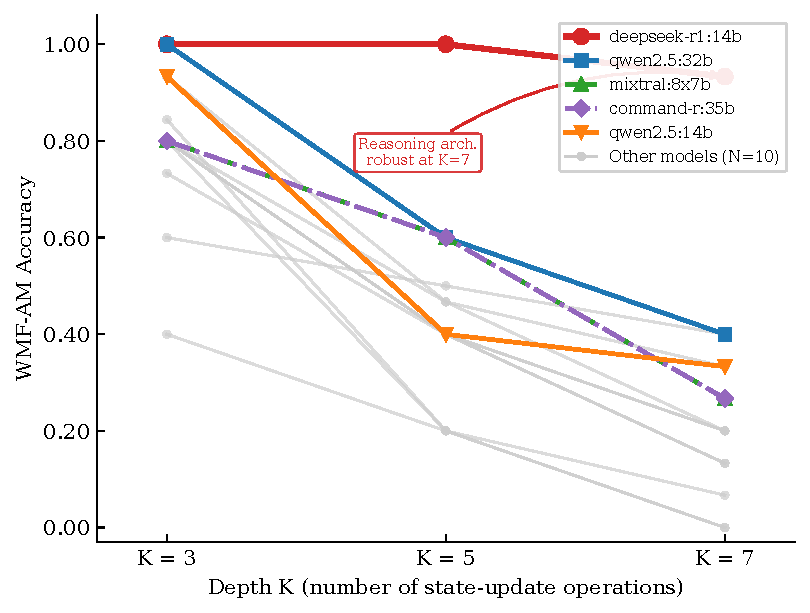
\includegraphics[width=0.72\textwidth]{fig2_depth_profile.pdf}
\caption{\textbf{WMF-AM accuracy by depth $K$ ($N{=}15$, chat template).}
deepseek-r1:14b (red) maintains near-perfect accuracy; all others
degrade sharply at $K \geq 5$. Top 5 models highlighted.}
\label{fig:depth}
\end{figure}

\subsection{Predictor Comparison and Exploratory Results}
\label{sec:exploratory}

Table~\ref{tab:predictor_comparison} shows WMF-AM against five predictors of ABS (see Appendix~\ref{app:protocols}
for the full 10-task table and battery release).
The yoked cancellation control (arithmetic parsing only: $\tau{=}{-}0.031$,
$p{=}0.879$) supports the interpretation that the predictive signal is specific to cumulative
state-tracking rather than arithmetic parsing ($\Delta\tau{=}0.491$, $p{=}0.022$).
Exploratory partial $\tau$
controlling for OC ($0.411$, $p{=}0.011$) and scale ($0.503$, $p{<}0.01$)
are hypothesis-generating; full details in Appendix~\ref{app:validity}.

\begin{table}[h]
\centering\small
\caption{\textbf{Predictor comparison: WMF-AM Score vs.\ alternative predictors of ABS.}
\textbf{C} = pre-specified; \textbf{E} = exploratory.
$\Delta\tau$ (WMF vs.\ Yoked): 0.491 ($p{=}0.022$, bootstrap, inferentially confirmed).
$\Delta\tau$ (WMF vs.\ OC/params): directional but not confirmed (95\% CI overlaps zero).}
\label{tab:predictor_comparison}
\resizebox{0.88\linewidth}{!}{%
\begin{tabular}{lcccc}
\toprule
\textbf{Predictor} & $\tau$ & $p$ & $N$ & \textbf{Note} \\
\midrule
\textbf{WMF-AM (this paper)} & \textbf{0.612} & \textbf{$<$0.001} & 20 & C \\
$\log(\text{params})$ & 0.444 & 0.010 & 20 & E \\
Outcome Correctness (OC) & 0.428 & 0.012 & 20 & E \\
$K{=}1$ single-step accuracy & 0.411 & 0.047 & 15 & E \\
Yoked cancellation accuracy & $-$0.031 & 0.879 & 15 & E (parsing only) \\
\bottomrule
\end{tabular}}
\end{table}

\subsection{Measurement Robustness}
\label{sec:meas_robustness}

Multi-seed reliability: all 15 models evaluated with 4 independent seeds
$\times$ 15 probes. Expansion-model SDs range 0.073--0.144 (mean 0.108),
comparable to original-model variability. Cross-template stability:
$\tau_{\text{bare,chat}} = 0.524$ ($p = 0.006$); $\tau_{\text{chat,cot}}
= 0.314$ ($p = 0.114$).
\textbf{Leave-one-family-out (exploratory):}
$\tau$ ranges 0.503--0.649 across family removals (mean 0.588); no
single family drives the effect.
\textbf{Family-aggregated (exploratory):}
Per-family median correlation $\tau = 0.538$ ($p = 0.030$, 13 families),
suggesting the relationship holds at the family level.
Full analyses in Appendix~\ref{app:robustness}.

\paragraph{Complementary probes (preliminary; Appendix~\ref{app:emclite}--\ref{app:ood}).}
Three probes at pilot scale ($N{\leq}8$, single seed):
EMC-lite ($\tau(\text{WMF-AM}){=}0.250$, consistent with independence);
MCC-CE-v2 (error rates 23--40\%, but 7/8 models show zero self-flagging);
CLA-DC (collapses onto WMF-AM, $\tau{=}0.905$, $N{=}7$).
No multi-dimensional structure claims are drawn from these pilots.

\subsection{Validity Summary}
\label{sec:validity}

Appendix~\ref{app:validity} gives the complete validity register.
\textbf{(Divergent, E)} WMF-AM $\leftrightarrow$ OC
$\tau{=}0.279$ ($p{=}0.150$, $N{=}15$); WMF$-$Yoked vs OC
$\tau{=}0.125$ ($p{=}0.519$), consistent with process--outcome independence.
\textbf{(Convergent, E)} CONV-RFPOC vs AGENT-PQ
$\tau{=}0.905$ ($N{=}7$; LLM judge; requires human annotation).
\textbf{(Template stability, C)} bare$\leftrightarrow$chat $\tau{=}0.524$
($p{=}0.006$).
Cross-dimension: CLA-DC collapses onto WMF-AM ($\tau{=}0.905$);
MCC-MA and EMC-lite remain separable.

% ─────────────────────────────────────────────────────────────────────────────
\section{Limitations, Alternative Views, and Discussion}
\label{sec:discussion}

\paragraph{Comparison to Minerva and K-calibration.}
Minerva~\citep{xia2025minerva} includes a Quantity State task at
$K{=}200$; all 20 study models score exactly 0.000, rendering $\tau$
undefined.
WMF-AM's $K{=}3/5/7$ calibration targets the discriminative window
(scores span $[0.050, 0.983]$; $\tau{=}0.619$ at $K{=}3$,
$0.509$ at $K{=}7$, undefined at $K{=}200$;
Appendix~\ref{app:ksweep}).
Beyond K-calibration, WMF-AM adds a construct-isolation ablation suite.

\paragraph{Key limitations.}
Limitations are organized by severity into four buckets.

\textbf{(L1) External validity (primary limitation).}
The sample comprises 20 open-weight models (0.5B--35B, greedy decoding,
Ollama variants); claims do not extend to closed API models, fine-tuned
variants, or non-English tasks. A single held-out check
(llama3.1:70b; $\tau{=}0.627$, $N{=}21$) is consistent with
but does not constitute replication.
The agent battery uses a single seed; multi-seed ABS reliability is
not established. Next step: extend to $N{\geq}30$ including API models.

\textbf{(L2) Construct validity.}
The $K{=}1$ control separates cumulative tracking from single-step
arithmetic; CoT collapses all models to ceiling ($\geq 0.93$), a
construct boundary.
Rival explanations (instruction-following, tokenizer effects) are
mitigated by cross-template stability ($\tau{=}0.524$) but not
eliminated (Appendix~\ref{app:rivals}).
A parsing artifact affects two verbose models (deepseek-r1:14b/7b);
88/90 responses contain the correct result.

\textbf{(L3) Sample size and dependence structure.}
$N{=}20$ supports the two pre-specified primary analyses but not factor
analysis; the four-dimension CEF structure is a provisional taxonomy,
not a validated empirical model. Family non-independence is substantial
(6 Qwen, 3 DeepSeek models); within-family ordering may trivially inflate
$\tau$. The within-Qwen robustness check ($\tau{=}0.894$, $p{=}0.016$,
$N{=}6$) is included but family-balanced sampling is needed for full rigor.

\textbf{(L4) Comparator scope.}
The completion proxy is a custom 100-item battery, not a standard
benchmark (MMLU, GSM8K). Partial-$\tau$ results controlling for
completion or scale are exploratory; held-out replication is needed.

\paragraph{What WMF-AM is not.}
Ablations indicate WMF-AM is unlikely to primarily measure general
arithmetic skill or working-memory capacity ($K{=}1$ control), generic
entity tracking (non-arithmetic ceiling), or arithmetic parsing
(yoked $\tau \approx 0$).
Instruction-following and tokenizer effects are mitigated by
cross-template stability but not eliminated; the mechanism linking
cumulative tracking difficulty to diverse agent tasks is not established.

\paragraph{Scope of contribution.}
WMF-AM is validated in one regime: open-weight models (0.5B--35B),
greedy decoding, no scratchpad.
The two pre-specified findings ($\tau{=}0.612$; $\tau{=}0.524$) are
in-sample evidence for this slice of model space; they do not
generalize to process-sensitive probes at large.
The CEF taxonomy is an organizing agenda, not an empirical result.

\paragraph{Implications.}
Evaluation suites would benefit from process probes alongside
completion: a load-varied probe~\citep{zhang2024working}, a
metacognitive component~\citep{lightman2023verify}, and a difficulty
gradient. Next steps: extend to API models ($N{\geq}30$), test against
standard benchmarks, and replicate across probe families.

\paragraph{Reproducibility.}
The 10-task agent battery, all WMF-AM probe templates, scoring scripts,
per-model raw outputs, and the pre-registered analysis plan
will be released upon publication at
\url{https://github.com/dengzhe-hou/CEF-WMF-AM}.

% ─────────────────────────────────────────────────────────────────────────────
\bibliographystyle{abbrvnat}
\bibliography{cef_refs}

% ═════════════════════════════════════════════════════════════════════════════
\appendix

\section{Full Motivation and Related Work}
\label{app:related_full}

\paragraph{Three failure modes of completion-only evaluation.}
\textbf{(F1) Diagnostic blindness}: models with near-identical completion
scores can have very different process profiles.
\textbf{(F2) Uninformative failure diagnosis}: current benchmarks report
\emph{that} an agent failed, not why, whether the bottleneck is
state tracking, metacognitive calibration, or episodic confusion.
\textbf{(F3) Safety blindness}: pattern-matching agents (which fail
predictably at distribution shift) are indistinguishable from genuine
reasoners on standard benchmarks.

{\sloppy
\paragraph{Empirical support.}
Multiple realizability is empirically documented at scale.
Fragile Thoughts~\citep{aravindan2026fragile} and Robust Answers
Fragile Logic~\citep{jiang2026robustanswersfragilelogic} show correct
answers produced despite corrupted reasoning.
Turpin et al.~\citep{turpin2023language} and Lanham et
al.~\citep{lanham2023measuring} show CoT can be systematically unfaithful.
PAE~\citep{xie2026m3}: 27--78\% of successful completions involve corrupted
intermediate actions.
AgentProcessBench~\citep{fan2026agentprocessbench}: 8,509-step human
annotation shows weaker models inflate correct-step ratios via early termination.
Chaduvula et al.~\citep{chaduvula2026features}: state-tracking inconsistency
is $2.7{\times}$ more prevalent in failed agent runs (TAU-bench).\par}

\paragraph{Positioning relative to prior work.}
Entity Tracking~\citep{entitytracking2023} is prior art for WMF-AM's design;
Latent State Persistence~\citep{huang2025language} probes sequential latent-state
manipulation on hidden integers, a closely related paradigm.
Minerva~\citep{xia2025minerva}: see Table~\ref{tab:minerva_compare}.
CEF adapts cognitive science measurement
logic~\citep{miller1956,baddeley1974,flavell1979,nelson1990,tulving1972episodic,sweller1988}
for API-level LLM evaluation without claiming LLMs have human cognition.
Process supervision~\citep{lightman2023verify,uesato2022solving}
trains models using step-level labels; CEF measures process quality.
Mechanistic interpretability explains why a score is low;
CEF identifies that it is low.

\begin{table}[h]
\centering
\small
\caption{\textbf{Comparison to Minerva Quantity State.}
WMF-AM does not claim benchmark superiority; it contributes
three additions to the existing arithmetic state-tracking paradigm.}
\label{tab:minerva_compare}
\resizebox{\linewidth}{!}{%
\begin{tabular}{lcc}
\toprule
\textbf{Property} & \textbf{Minerva QS} & \textbf{WMF-AM (this paper)} \\
\midrule
Arithmetic state-tracking task & \checkmark & \checkmark \\
Step-count variation & \checkmark ($K$ variable) & \checkmark ($K{=}3,5,7$) \\
Calibrated for open-weight discriminability & $\times$ (K=200: 20/20 models floor at 0.000) & \checkmark ($K{=}3/5/7$: range [0.050, 0.983]) \\
Construct-isolation ablation suite & $\times$ & \checkmark (yoked, $K{=}1$, non-arith) \\
Downstream predictive validity & $\times$ & \checkmark ($\tau{=}0.612$, N=20) \\
Kendall $\tau$ with agent performance & undefined (constant) & \textbf{0.612} ($p{<}0.001$) \\
Multi-seed + multi-template stability & $\times$ & \checkmark \\
Head-to-head on same 20 models & N/A & \checkmark (this paper) \\
\bottomrule
\end{tabular}}
\end{table}

\section{K-Sweep: Discriminability vs.\ Step Count}
\label{app:ksweep}

\begin{table}[h]
\centering\small
\caption{\textbf{K-sweep: discriminability vs.\ step count.}
$\tau{=}\tau(\text{probe}, \text{Agent})$; $N$ = models with per-K data.
K=3--7: WMF-AM per-depth means (N=12 models for which per-K breakdowns were collected; the remaining 8 were tested only at the composite level); K=20: 5-model inline test;
K=200: full 20-model head-to-head.}
\label{tab:ksweep}
\resizebox{0.82\linewidth}{!}{%
\begin{tabular}{cccccc}
\toprule
$K$ & $N$ & Mean acc & Range & $\tau$ & $p$ \\
\midrule
3 & 12 & 0.512 & $[0.050, 0.950]$ & \textbf{0.619} & 0.007 \\
5 & 12 & 0.296 & $[0.000, 1.000]$ & \textbf{0.545} & 0.020 \\
7 & 12 & 0.192 & $[0.000, 1.000]$ & \textbf{0.509} & 0.032 \\
20 & 5  & 0.180 & $[0.000, 0.900]$ & $-$0.333 & 0.47 \\
200 (Minerva) & 20 & 0.000 & $[0.000, 0.000]$ & undef & undef \\
\bottomrule
\end{tabular}}
\end{table}

\section{CEF Framework Background}
\label{app:cef_background}

CEF (Cognitive Evaluation Framework) organizes process-sensitive probes
into four proposed dimensions: WMF (Working Memory Fidelity, 3 sub-dimensions),
MCC (Metacognitive Calibration, 2), EMC (Episodic Memory Coherence, 3),
and CLA (Cognitive Load Adaptation, 3). Each dimension has a cognitive science
anchor, a documented evaluation gap, and API-level testability.
Labels like ``working memory'' are operational shorthand, not
mechanistic claims (see Appendix~\ref{app:labels}).
Figure~\ref{fig:framework} illustrates the taxonomy and
Table~\ref{tab:dims} summarizes the four dimensions.

\begin{figure}[h]
\centering
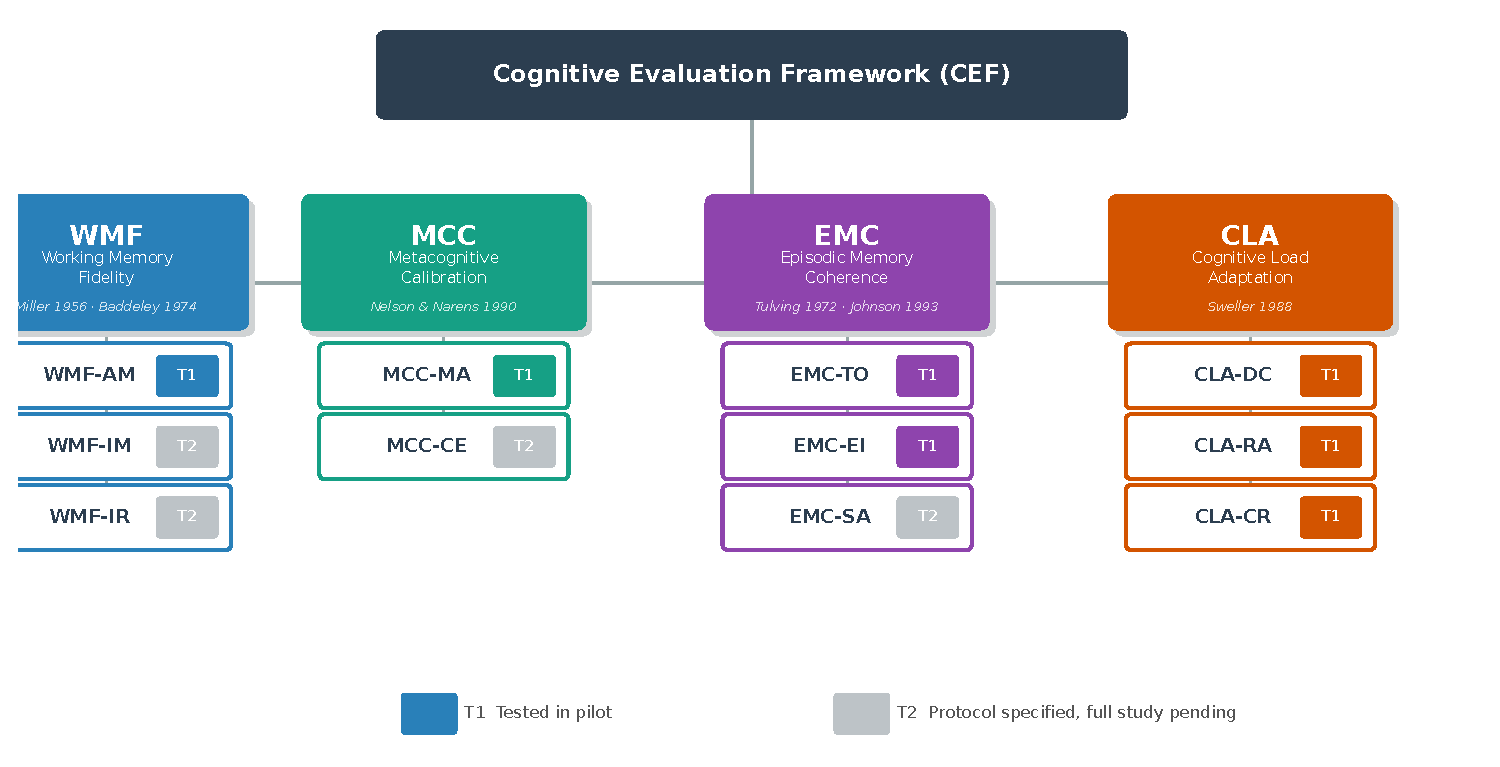
\includegraphics[width=0.85\textwidth]{fig3_framework.pdf}
\caption{\textbf{CEF taxonomy.} Four proposed dimensions (WMF, MCC, EMC, CLA)
with sub-dimensions, cognitive anchors, and probe mappings.
Only WMF-AM is empirically validated in this paper; other dimensions
are included as design context.}
\label{fig:framework}
\end{figure}

\begin{table}[h]
\centering
\small
\caption{CEF dimensions: target, failure signature, and exclusions.
Detailed sub-dimension definitions appear in Appendix~\ref{app:subdims}.}
\label{tab:dims}
\resizebox{\linewidth}{!}{%
\begin{tabular}{lp{3cm}p{3cm}p{3cm}}
\toprule
\textbf{Dim} & \textbf{Target} & \textbf{Failure signature} & \textbf{Excluded} \\
\midrule
WMF & Active maintenance and transformation of state under load
  & Accuracy drops as concurrent items exceed threshold
  & Long-context retrieval; knowledge recall \\
MCC & Self-monitoring of errors (MA) and correction of flagged errors (CE)
  & Confident-wrong; flagging without correction
  & General calibration (ECE); cross-model detection \\
EMC & Temporal ordering, cross-episode discrimination, source attribution
  & Episode blending; source misattribution
  & Single-turn retrieval; semantic memory \\
CLA & Degradation shape and resource scaling under load
  & Cliff-edge failure; non-recovery
  & Knowledge difficulty; unrelated complexity \\
\bottomrule
\end{tabular}}
\end{table}

\paragraph{Other CEF dimensions (background; not validated in this paper).}
\textbf{MCC}: decomposes metacognition into monitoring accuracy (MCC-MA)
and control efficacy (MCC-CE).
\textbf{EMC}: tests temporal ordering, cross-episode discrimination,
and source attribution under interference.
\textbf{CLA}: characterizes the performance-versus-load function shape;
CLA-DC provisionally collapses onto WMF-AM ($\tau{=}0.905$, $N{=}7$)
pending factor analysis at $N{\geq}20$.

\paragraph{Construct validity framework.}
Following~\citet{cronbach1955construct}, \citet{messick1989validity},
\citet{campbell1959convergent}, and \citet{jacobs2021measurement},
each dimension requires convergent validity (correlation with independent
process-sensitive measures) and divergent validity (low correlation with
completion). The study supports divergent validity for WMF-AM
($\tau = 0.279$ with a 100-item completion battery, $N{=}15$).
CEF would be falsified if all dimensions collapsed onto a single factor
indistinguishable from task completion.
Figure~\ref{fig:validity} visualizes the validity evidence across probes,
and Appendix~\ref{app:falsify} provides full construct-to-probe mapping.

\begin{figure}[h]
\centering
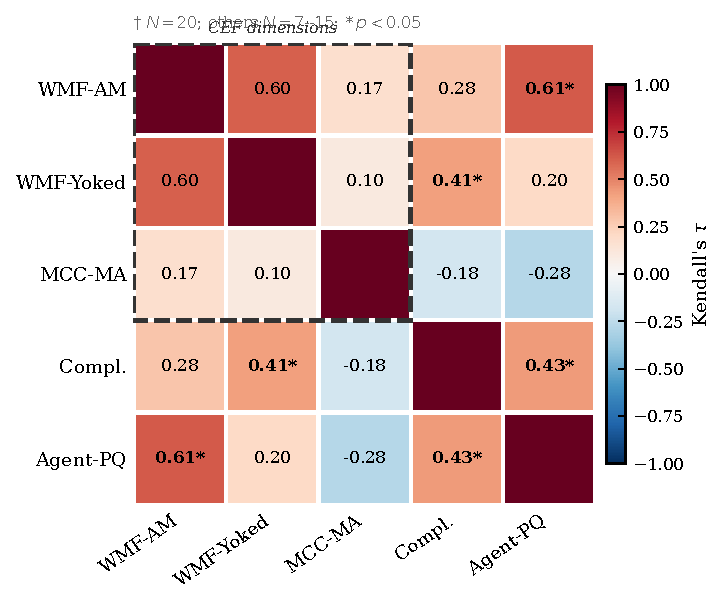
\includegraphics[width=0.78\textwidth]{fig4_validity_heatmap.pdf}
\caption{\textbf{Validity evidence heatmap.} Convergent and divergent
correlations across CEF probes and external benchmarks ($N{=}15$).
WMF-AM shows high divergent validity (low correlation with completion)
and moderate convergent validity with agent battery scores.}
\label{fig:validity}
\end{figure}

\section{Full Related Work Table}
\label{app:related}

\begin{table}[h]
\centering
\small
\caption{Representative benchmarks and evaluation work, grouped by
measurement type and CEF gap addressed.}
\label{tab:benchmarks}
\resizebox{\linewidth}{!}{%
\begin{tabular}{@{}llp{7cm}@{}}
\toprule
\textbf{Work} & \textbf{Measures} & \textbf{CEF gap addressed} \\
\midrule
MMLU~\citep{hendrycks2021mmlu}, ARC~\citep{clark2018arc}, HellaSwag~\citep{zellers2019hellaswag} & Knowledge recall & No memory structure, no process \\
HumanEval~\citep{chen2021humaneval}, MATH~\citep{hendrycks2021math}, GSM8K~\citep{cobbe2021gsm8k} & Output correctness & No reasoning fidelity \\
HotpotQA~\citep{yang2018hotpotqa}, WebShop~\citep{yao2022webshop} & Task completion & No metacognition, no memory type differentiation \\
AgentBench~\citep{liu2023agentbench} & Sequential task success & No within-task process \\
Reflexion~\citep{shinn2023reflexion} & Post-reflection improvement & Monitoring $\neq$ control (conflated) \\
PAE~\citep{xie2026m3} & Corruption rate & Motivates CEF; no per-dimension measurement \\
NeuroCognition~\citep{haznitrama2026neuropsychologicallygroundedevaluationllm} & Cognitive ability (IQ) & Ability $\neq$ process quality; no load variation \\
Strong Mem.\ \& Weak Ctrl.~\citep{de2025strong} & Executive function & Isolated tasks; no multi-turn load \\
Entity Tracking~\citep{entitytracking2023} & Entity-state & Prior art for WMF-AM design (passive retrieval) \\
Latent State Persistence~\citep{huang2025language} & Sequential latent-state manipulation & Closest prior paradigm; no arithmetic load, no agent battery \\
Minerva~\citep{xia2025minerva} & Programmable memory (incl.\ Quantity State: sequential +/-) & Closest arithmetic prior; WMF-AM adds construct-isolation suite + agent-predictive validity \\
Zhang et al.~\citep{zhang2024working} & WM-style probes → reasoning limits & Motivational; no ablation suite, no agent battery \\
Intell.\ Degradation~\citep{wang2026intelligence} & Load degradation & Prior art for CLA \\
HELM~\citep{liang2023helm} & Behavioral outcomes & No cognitive processes \\
Long-context~\citep{bai2024longbench} & Retrieval from static window & WMF-AM targets active transformation \\
ECE calibration~\citep{guo2017calibration} & Confidence scalar & MCC decomposes into monitoring/control \\
\bottomrule
\end{tabular}}
\end{table}

\section{Development Status and Summary Tables}
\label{app:tables}

\begin{table}[h]
\centering
\footnotesize
\caption{\textbf{Development status of all 11 CEF sub-dimensions.}
Status key \textbf{A}: robust differentiation + multi-seed reliability;
\textbf{B}: differentiation shown, limited seeds/models;
\textbf{C}: probe redesigned, initial results;
\textbf{D}: ceiling/floor effect, needs redesign;
\textbf{E}: protocol specified, no pilot data.}
\label{tab:valstatus}
\resizebox{\linewidth}{!}{%
\begin{tabular}{@{}llll@{}}
\toprule
\textbf{Sub-dim} & \textbf{Status} & \textbf{Evidence} & \textbf{Limitation} \\
\midrule
WMF-AM & A$^+$ & $\Delta{=}0.933$, 4-seed all 20, 3-template ($\tau{=}0.524$), yoked control, predictive $\tau{=}0.612$ & All open-weight \\
WMF-IM & B & spread 0.480, $N{=}5$ & Single paradigm (hard) \\
WMF-IR & D & Ceiling ($= 1.0$ all models) & Needs redesign \\
MCC-MA & B & 4/7 models differentiated & Floor for 3 models \\
MCC-CE & C & v2: error 23--40\%, near-zero flagging ($N{=}8$) & Binary protocol \\
EMC-lite & B & Source-conflict spread 0.400 & Single seed \\
CLA-DC & B$^\dagger$ & Correlates $\tau{=}0.905$ with WMF-AM & $^\dagger$Provisionally collapsed onto WMF \\
CLA-CR & C & v3 spread 1.171, $N{=}7$ & v1--v2 failed; 2 seeds \\
CLA-RA & E & --- & Awaits full study \\
EMC-TO & E & --- & Awaits full study \\
EMC-EI & E & --- & Awaits full study \\
\bottomrule
\end{tabular}}
\end{table}

\begin{table}[h]
\centering
\footnotesize
\caption{\textbf{CEF at a glance.} Each sub-dimension's task type, scoring
rule, and pilot status. Tier 1 = novel construct; Tier 2 = novel
reframing. Pilot: \checkmark\,= pilot-supported, $\sim$\,= preliminary,
---\,= protocol only.}
\label{tab:ataglance}
\resizebox{\linewidth}{!}{%
\begin{tabular}{@{}llllc@{}}
\toprule
\textbf{Sub-dim} & \textbf{Task (one-line)} & \textbf{Scoring} & \textbf{Tier} & \textbf{Pilot} \\
\midrule
WMF-AM & Track $K$ sequential state updates, report final state & Exact match & 1 & \checkmark \\
WMF-IM & Recall $N$ facts amid $M$ distractors & Recall accuracy & 2 & $\sim$ \\
WMF-IR & Recall List-A after List-B interference & Proactive interference $\delta$ & 2 & --- \\
MCC-MA & Predict which of 20 answers are wrong & Pearson $r$ (predicted vs.\ actual) & 1 & $\sim$ \\
MCC-CE & Flag uncertain answers, revise them & Correction efficacy & 1 & $\sim$ \\
EMC-TO & Reorder non-chronological events & Kendall $\tau$ vs.\ ground truth & 1 & --- \\
EMC-EI & Discriminate similar episodes & Accuracy under similarity & 1 & --- \\
EMC-SA & Attribute facts to source + episode & Joint attribution accuracy & 2 & --- \\
CLA-DC & Performance across 5 load levels & Smoothness (SD of $\Delta$s) & 1 & --- \\
CLA-RA & Response elaboration vs.\ difficulty & Pearson $r$ & 1 & --- \\
CLA-CR & Easy-task recovery after high-load block & Recovery rate & 1 & $\sim$ \\
\bottomrule
\end{tabular}}
\end{table}

\section{Glossary}
\label{app:glossary}

\begin{table}[h]
\centering
\footnotesize
\caption{Glossary of key terms and acronyms.}
\label{tab:glossary}
\begin{tabular}{@{}lp{9cm}@{}}
\toprule
\textbf{Term} & \textbf{Definition} \\
\midrule
CEF & Cognitive Evaluation Framework (this paper) \\
WMF-AM/IM/IR & Working Memory Fidelity: Active Manipulation / Information Maintenance / Interference Resistance \\
MCC-MA/CE & Metacognitive Calibration: Monitoring Accuracy / Control Efficacy \\
EMC-TO/EI/SA & Episodic Memory Coherence: Temporal Ordering / Episodic Interference / Source Attribution \\
CLA-DC/RA/CR & Cognitive Load Adaptation: Degradation Curve / Resource Allocation / Capacity Recovery \\
AGENT-PQ/TC & Agent Process Quality / Task Completion (external evaluation) \\
CONV-RFPOC & Convergent validity probe: Reasoning Fidelity--Product of Cognition \\
\bottomrule
\end{tabular}
\end{table}

\section{On Cognitive-Science Labels}
\label{app:labels}

We use labels like ``working memory'' and ``metacognition'' as
operational shorthand for specific behavioral probes, not as
claims about LLM internal mechanisms. ``WMF-AM'' means: ``accuracy on
sequential state-tracking tasks degrades with depth $K$''; it does not
mean LLMs have a working memory buffer. ``MCC-MA'' means: ``accuracy
of self-error prediction on a 20-item probe''; it does not mean LLMs
have phenomenal metacognition. The labels are justified because the
probes are adapted from validated human measurement paradigms, and they
organize what would otherwise be an unstructured collection of tests.

Two caveats are essential. First, we do not require LLMs to have
phenomenal cognition or internal states analogous to human working memory.
CEF dimensions are process-sensitive behavioral probes that borrow
measurement logic from cognitive science. Second, CEF measurements are
behavioral (prompt/response), designed to be differentially sensitive to
process quality: high MCC-MA requires accurate self-error prediction;
graceful CLA-DC requires proportional rather than catastrophic
degradation.

\section{Full Sub-dimension Definitions}
\label{app:subdims}

\paragraph{WMF-AM (Active Manipulation, Tier 1).}
Uses a complex span task: initial state, $K$ sequential modifications,
report final state. Depths $K \in \{3,5,7\}$ (dissociation study) and
$K \in \{2,4,6,8,12\}$ (yoked cancellation control), three surface forms.
Prior entity tracking~\citep{entitytracking2023} tests passive retrieval;
WMF-AM tests sequential transformation.

\paragraph{WMF-IM (Information Maintenance, Tier 2).}
Embeds $N$ facts in a passage with $M$ distractors; measures recall
accuracy. Extends Wang and Sun~\citep{wang2025unableforgetproactiveinterference}
to natural-language multi-turn contexts.

\paragraph{WMF-IR (Interference Resistance, Tier 2).}
Adapts the List-A/List-B proactive interference paradigm.
Currently shows ceiling ($= 1.0$ all models); needs redesign.

\paragraph{MCC-MA (Monitoring Accuracy, Tier 1).}
Model predicts which of 20 answers are incorrect; Pearson $r$ measures
monitoring accuracy. Unlike Gnosis~\citep{ghasemabadi2025can} (requires
internals), MCC-MA uses prompting under multi-turn load.

\paragraph{MCC-CE (Control Efficacy, Tier 1).}
Model flags uncertain answers and revises them. Decomposes into flagging
rate, correction efficacy, and false alarm rate.

\paragraph{EMC-TO/EI/SA.}
Temporal ordering (Kendall $\tau$), cross-episode discrimination under
similarity, and joint source-episode attribution. All proposed, no pilot data.

\paragraph{CLA-DC (Degradation Curve, Tier 1).}
Smoothness score (SD of successive $\Delta$s). Provisionally collapsed
onto WMF-AM ($\tau = 0.905$).

\paragraph{CLA-RA/CR.}
Resource allocation (difficulty--elaboration correlation) and capacity
recovery (post-load accuracy recovery). CLA-RA has no pilot data;
CLA-CR-v3 spread $= 1.171$.

\paragraph{Composites (all exploratory).}
$\text{WMF} = 0.50 \times \text{AM} + 0.30 \times \text{IM} + 0.20 \times \text{IR}$;
$\text{MCC} = 0.55 \times \text{MA} + 0.45 \times \text{CE}$;
$\text{EMC} = 0.40 \times \text{EI} + 0.35 \times \text{TO} + 0.25 \times \text{SA}$;
$\text{CLA} = 0.50 \times \text{DC} + 0.30 \times \text{RA} + 0.20 \times \text{CR}$.
We do \emph{not} propose an overall CEF composite; per-dimension profiles
are the primary unit of analysis.

\section{Construct-to-Probe Mapping and Falsifiability}
\label{app:falsify}

The framework as a whole would be undermined if process-sensitive
measures never provided incremental prediction beyond completion
on any downstream criterion.
Table~\ref{tab:falsify} specifies per-probe falsification conditions.

\begin{table}[h]
\centering
\footnotesize
\caption{Construct map for validated probes: manipulated factor,
observable signature, rival explanations, and falsification criteria.}
\label{tab:falsify}
\resizebox{\linewidth}{!}{%
\begin{tabular}{@{}lp{2cm}p{2cm}p{2.5cm}p{2.5cm}p{2.5cm}@{}}
\toprule
\textbf{Probe} & \textbf{Manipulated factor} & \textbf{Observable signature} & \textbf{Plausible rivals} &
\textbf{Expected pattern} & \textbf{Falsified if} \\
\midrule
WMF-AM & Depth $K$ (number of sequential state updates) &
  Accuracy $\times$ depth interaction &
  Instruction following; tokenizer parsing; template familiarity; long-context retrieval &
  Low $\tau$ with completion; monotonic depth decline; $\tau_{\text{bare,chat}} > 0.4$; yoked control $\gg$ WMF-AM &
  High $\tau$ with completion ($\geq 0.55$); no depth effect; template-specific rankings; control degrades at same rate \\
MCC-MA & Error-laden vs correct items &
  Pearson $r$ (predicted vs actual errors) &
  Calibration shortcuts; always-predict-correct bias &
  Low $\tau$ with WMF-AM; model-specific prediction &
  Uniform predictions; $\tau \approx 1$ with WMF-AM \\
EMC-lite & Conflict vs control episodes &
  Source attribution accuracy under interference &
  Recency bias; keyword matching &
  Low $\tau$ with WMF-AM; fault $>$ control difficulty &
  No fault--control difference; $\tau \approx 1$ with WMF-AM \\
\bottomrule
\end{tabular}}
\end{table}

\section{Rival Explanations}
\label{app:rivals}

For each probe, plausible alternative explanations remain open.
\textbf{WMF-AM:} (a) Instruction following: models may fail at
depth because they lose track of instructions. The depth gradient partly
addresses this.
(b) Long-context retrieval: the control addresses this for 5/7
models.
(c) Template artifacts: cross-template stability
(bare$\leftrightarrow$chat $\tau{=}0.524$, $p{=}0.006$; paraphrase
original-vs-formal $\tau{=}0.857$) mitigates but does not eliminate this.
\textbf{MCC-MA/CE:} (a)~Calibration shortcuts. (b)~Prompt sensitivity.
\textbf{EMC-lite:} Recency bias; keyword matching.
These are the primary targets for the $N \geq 15$ study.

\section{Study Matrix}
\label{app:studymatrix}

\begin{table}[h]
\centering
\footnotesize
\caption{Study matrix: all experiments, models, and sample sizes.
$^\dagger$llama3.1:70b added for MCC-CE-v2 only.}
\label{tab:studymatrix}
\begin{tabular}{@{}llccc@{}}
\toprule
\textbf{Experiment} & \textbf{Metric} & $N_\text{models}$ & \textbf{Seeds} & \textbf{Trials/model} \\
\midrule
Outcome Correctness (v2) & Accuracy & 20 & 1 & 100 \\
WMF-AM (dissociation) & Exact match & 20 & 4 & 180 \\
Agent Validation & Deterministic task score & 20 & 1 & 10 \\
Template Harmonization & Rank stability & 15 & 1 & 135 \\
Yoked Cancellation Control & Exact match & 15 & 1 & 100 \\
MCC-MA & Pearson $r$ & 15 & 1 & 20 \\
MCC-CE-v2 & Flagging rate & 8$^\dagger$ & 1 & 50 \\
EMC-lite & Composite & 7 & 1 & 18 \\
CLA-CR-v3 & Recovery rate & 7 & 2 & 7 blocks \\
AGENT-PQ/TC & Rubric / binary & 7 & 1 & 10 \\
CONV-RFPOC & Fidelity & 7 & 1 & 15 \\
\bottomrule
\end{tabular}
\end{table}

\section{Yoked Cancellation Control Details}
\label{app:control}

The yoked cancellation control uses operation pairs that cancel:
``Alice gains 3 points'' followed immediately by ``Alice loses 3 points.''
The prompt format, entity names, and depth structure match WMF-AM exactly,
so the arithmetic parsing demand is identical. The correct answer equals
the initial state, but unlike the original inert control, the model must
process each operation to verify cancellation. This eliminates the
trivial shortcut of ignoring operations.

\section{Measurement Robustness}
\label{app:robustness}

\paragraph{Multi-seed reliability.}
All 15 models evaluated with 4 independent random seeds $\times$ 15
probes. Original-model cross-seed $\tau = 0.798$. Expansion-model SDs:
phi3:14b $= 0.094$, gemma2:9b $= 0.144$, qwen2.5:3b $= 0.122$,
llama3.2:3b $= 0.122$, deepseek-r1:7b $= 0.114$, mixtral:8x7b $= 0.116$,
command-r:35b $= 0.100$, yi:34b $= 0.084$ (mean SD $= 0.108$).

\paragraph{Cross-template stability.}
Phase~5 administered WMF-AM under three prompt wrappers (bare, chat,
chain-of-thought) across all 15 models.
Bare $\leftrightarrow$ chat: $\tau = 0.524$ ($p = 0.006$), significant
rank preservation.
Bare $\leftrightarrow$ CoT: $\tau = 0.105$ ($p = 0.627$), CoT pushes
all models to ceiling ($\geq 0.93$), eliminating variance.
Chat $\leftrightarrow$ CoT: $\tau = 0.314$ ($p = 0.114$).
The CoT ceiling effect is interpretively meaningful: externalized
reasoning via scratchpad bypasses the working-memory bottleneck that
WMF-AM is designed to measure.

\paragraph{Non-ceiling completion proxies.}
$\tau(\text{WMF-AM, MMLU}) = 0.356$ ($p = 0.317$; range 0.25--0.72);
$\tau(\text{WMF-AM, GSM8K}) = 0.150$ ($p = 0.645$; range 0.05--0.83).
Scores from published model cards, not re-evaluated under pilot setup.

\paragraph{Depth profile.}
See Figure~\ref{fig:depth} in the main text for depth-dependent degradation curves.

\section{EMC-lite Results}
\label{app:emclite}

\begin{table}[h]
\centering
\small
\caption{\textbf{EMC-lite ($N{=}7$, hardened protocol).}
Source attribution shows strongest differentiation (spread $= 0.500$).}
\label{tab:emclite}
\begin{tabular}{lcccccc}
\toprule
Model & F-Det & F-Src & F-Rec & F-Comp & C-Rec & $\Delta$Rec \\
\midrule
qwen2.5:14b     & 0.917 & 0.750 & 0.917 & \textbf{0.917} & 0.972 & $-$0.056 \\
qwen2.5:32b     & 0.917 & 0.750 & 0.917 & \textbf{0.917} & 1.000 & $-$0.083 \\
deepseek-r1:14b & 0.889 & \textbf{0.917} & 0.917 & 0.912 & 1.000 & $-$0.083 \\
llama3.1:8b     & 0.778 & 0.583 & 0.750 & 0.771 & 0.889 & $-$0.139 \\
qwen2.5:7b      & 0.861 & 0.583 & 0.639 & 0.736 & 0.722 & $-$0.083 \\
mistral:7b      & 0.750 & \textbf{0.417} & 0.639 & 0.685 & 0.722 & $-$0.083 \\
gemma2:27b      & 0.861 & 0.583 & 0.528 & 0.667 & 0.611 & $-$0.083 \\
\midrule
$\Delta$ & 0.167 & \textbf{0.500} & 0.389 & \textbf{0.250} & 0.389 & — \\
\bottomrule
\end{tabular}
\end{table}

EMC-lite provides preliminary support for the source-conflict slice.
It does not establish EMC as a whole; single-seed evidence only.
$\tau(\text{WMF-AM, EMC-lite}) = 0.250$: substantial independence.

\section{MCC-CE-v2 Results}
\label{app:mccv2}

\begin{table}[h]
\centering
\small
\caption{\textbf{MCC-CE-v2 ($N{=}8$).} Error rates 23--40\% (floor
eliminated); flagging near zero for all models.}
\label{tab:mcc_v2}
\begin{tabular}{lcc|cc}
\toprule
& \multicolumn{2}{c|}{\textbf{Balanced ($n{=}30$)}} & \multicolumn{2}{c}{\textbf{Trap-only ($n{=}20$)}} \\
\textbf{Model} & Error\% & Flag\% & Error\% & Flag\% \\
\midrule
qwen2.5:7b      & 26.7 & 0.0 & 40.0 & 0.0 \\
qwen2.5:14b     & 36.7 & 0.0 & 40.0 & 0.0 \\
qwen2.5:32b     & 30.0 & 0.0 & 25.0 & 0.0 \\
llama3.1:8b     & 26.7 & 0.0 & 40.0 & 0.0 \\
llama3.1:70b    & ---  & --- & 25.0 & 0.0 \\
gemma2:27b      & 30.0 & \textbf{11.1} & 30.0 & 0.0 \\
deepseek-r1:14b & 23.3 & 0.0 & 35.0 & 0.0 \\
mistral:7b      & 30.0 & 0.0 & 40.0 & 0.0 \\
\bottomrule
\end{tabular}
\end{table}

The v1 floor was an artifact of easy questions; v2 models make many
errors but show near-zero self-flagging under the binary protocol.
Alternative designs (continuous confidence, forced ranking) might reveal
partial capacity.

\section{Negative OOD Result}
\label{app:ood}

Two OOD stress-test designs (v1: 5-step NL tasks; v2: $K{=}8$--$9$
interference tasks) produced anti-correlated CEF--OOD relationships
across model pairs. We make no predictive claim. Full assessment requires
$N \geq 11$ with process-sensitive downstream tasks.

\section{Full Validity Analyses}
\label{app:validity}

Below we provide additional details on the validity analyses summarized in Section~\ref{sec:validity}.

\paragraph{Convergent validity details.}
AGENT-PQ: 10 multi-step scenarios scored by LLM judge (GPT-4o) on
4 rubric dimensions. CONV-RFPOC: 15 reasoning problems with
counterfactual chain perturbation. RFPOC $= 1 - P(\text{same answer}
\mid \text{perturbed chain})$. Full protocol in
Appendix~\ref{app:agentpq}.
\textbf{Limitation:} LLM judge may introduce shared bias.

\paragraph{Construct separation (WMF-AM $\leftrightarrow$ CLA-DC).}
$\tau = 0.905$: no evidence of separability at $N{=}7$. Both involve
state tracking under load. Planned discriminant test at $N \geq 15$.
CLA-CR-v3 provides a structurally independent CLA measure.
Even if CLA-DC merges with WMF-AM, WMF-AM, MCC-MA, and EMC-lite
remain separable ($\tau \leq 0.250$).

\paragraph{Sensitivity.}
LOMO for CONV-RFPOC vs AGENT-PQ: $\tau$ ranges 0.600--1.000
(mean 0.833). Leave-one-family-out (Qwen, $N{=}4$): $\tau = 0.667$.
After Holm correction, RFPOC--AGENT-PQ remains significant
($p_\text{adj} = 0.021$).

\paragraph{Multiple testing.}
Two primary hypotheses; all others exploratory.

\paragraph{Benchmark governance.}
All headline results use frozen protocol versions. Probe revisions were
motivated by floor/ceiling effects, not model-specific tuning.

\section{AGENT-PQ Evaluation Protocol}
\label{app:agentpq}

\textbf{AGENT-PQ} uses 10 multi-step scenarios where each model operates
within a tool-use scaffold. A separate LLM judge (GPT-4o, temperature
$= 0$) scores each trajectory on four rubric dimensions:
plan coherence, state tracking, error recovery, goal adherence.
AGENT-PQ $= \text{mean of 4 rubric scores} / 4$.
AGENT-TC is the binary success rate on the same scenarios.

\textbf{CONV-RFPOC} administers 15 reasoning problems with
counterfactual chain perturbation.
RFPOC $= 1 - P(\text{same answer} \mid \text{perturbed chain})$.

\section{Complete Experimental Protocols}
\label{app:protocols}

Full prompt templates, parameter specifications, scoring procedures, and
reference implementations for all 11 sub-dimensions are provided in the
supplementary materials.

\section{Weight Sensitivity Analysis}
\label{app:weights}

Three weighting schemes (proposed, equal, PCA-derived) are evaluated.
Per-dimension profiles are primary; composites are exploratory only.

\section{Dissociation Case Studies}
\label{app:dissociation}

Matched dissociation pairs: deepseek-r1:14b and qwen2.5:14b share
similar EMC-lite (0.912 vs.\ 0.917) but differ on WMF-AM (0.983 vs.\
0.467). mistral:7b and llama3.1:8b have similar WMF-AM but differ on
EMC-lite. These cross-dimension pairs anchor the multiple realizability
argument.

\section{Worked Example: WMF-AM at Depth $K{=}3$}
\label{app:worked}

\noindent\textbf{Setup.} ``A warehouse has 3~items: Widget=50,
Gadget=30, Sprocket=20.'' Three updates: ``Ship 10~Widgets,''
``Receive 25~Gadgets,'' ``Transfer 5~Sprockets to overflow.''

\noindent\textbf{Correct.} Widget=40, Gadget=55, Sprocket=15.

\noindent\textbf{Scoring.} Exact match per item. deepseek-r1:14b scores
1.000 at $K{=}7$; llama3.1:8b scores 0.050. Both score 0.90--0.95 on
outcome correctness. This illustrates the Completion Fallacy.

\section{Novelty Classification}
\label{app:novelty}

\begin{table}[h]
\centering
\small
\caption{Novelty tier for all 11 sub-dimensions. Tier 1 = novel;
Tier 2 = novel reframing.}
\label{tab:novelty}
\begin{tabular}{llp{6.5cm}}
\toprule
\textbf{Sub-dim} & \textbf{Tier} & \textbf{Prior art / differentiation} \\
\midrule
WMF-AM & 1 & Entity Tracking~\citep{entitytracking2023}: passive retrieval; Latent State Persistence~\citep{huang2025language}: structural ops, no arithmetic load, no agent battery; WMF-AM = cumulative arithmetic transformation + ablation suite + downstream validity \\
WMF-IM & 2 & Wang \& Sun~\citep{wang2025unableforgetproactiveinterference}: key-value pairs; WMF-IM = NL multi-turn \\
WMF-IR & 2 & Extended to domain-varied materials \\
MCC-MA & 1 & Gnosis~\citep{ghasemabadi2025can} requires internals; MCC-MA = prompting only \\
MCC-CE & 1 & Reflexion~\citep{shinn2023reflexion}: aggregate; MCC-CE decomposes detection/correction \\
EMC-TO & 1 & No prior LLM temporal ordering measurement \\
EMC-EI & 1 & No prior cross-episode interference diagnostic \\
EMC-SA & 2 & Interference-conditioned attribution \\
CLA-DC & 1 & Intell.\ Degradation~\citep{wang2026intelligence}: magnitude; CLA-DC = shape \\
CLA-RA & 1 & Not previously measured \\
CLA-CR & 1 & Not previously measured \\
\bottomrule
\end{tabular}
\end{table}

\end{document}